\section{Optimal Control of Pitch/Travel without Feedback}\label{sec:prob2}

\begin{figure}[hp]
	\centering
		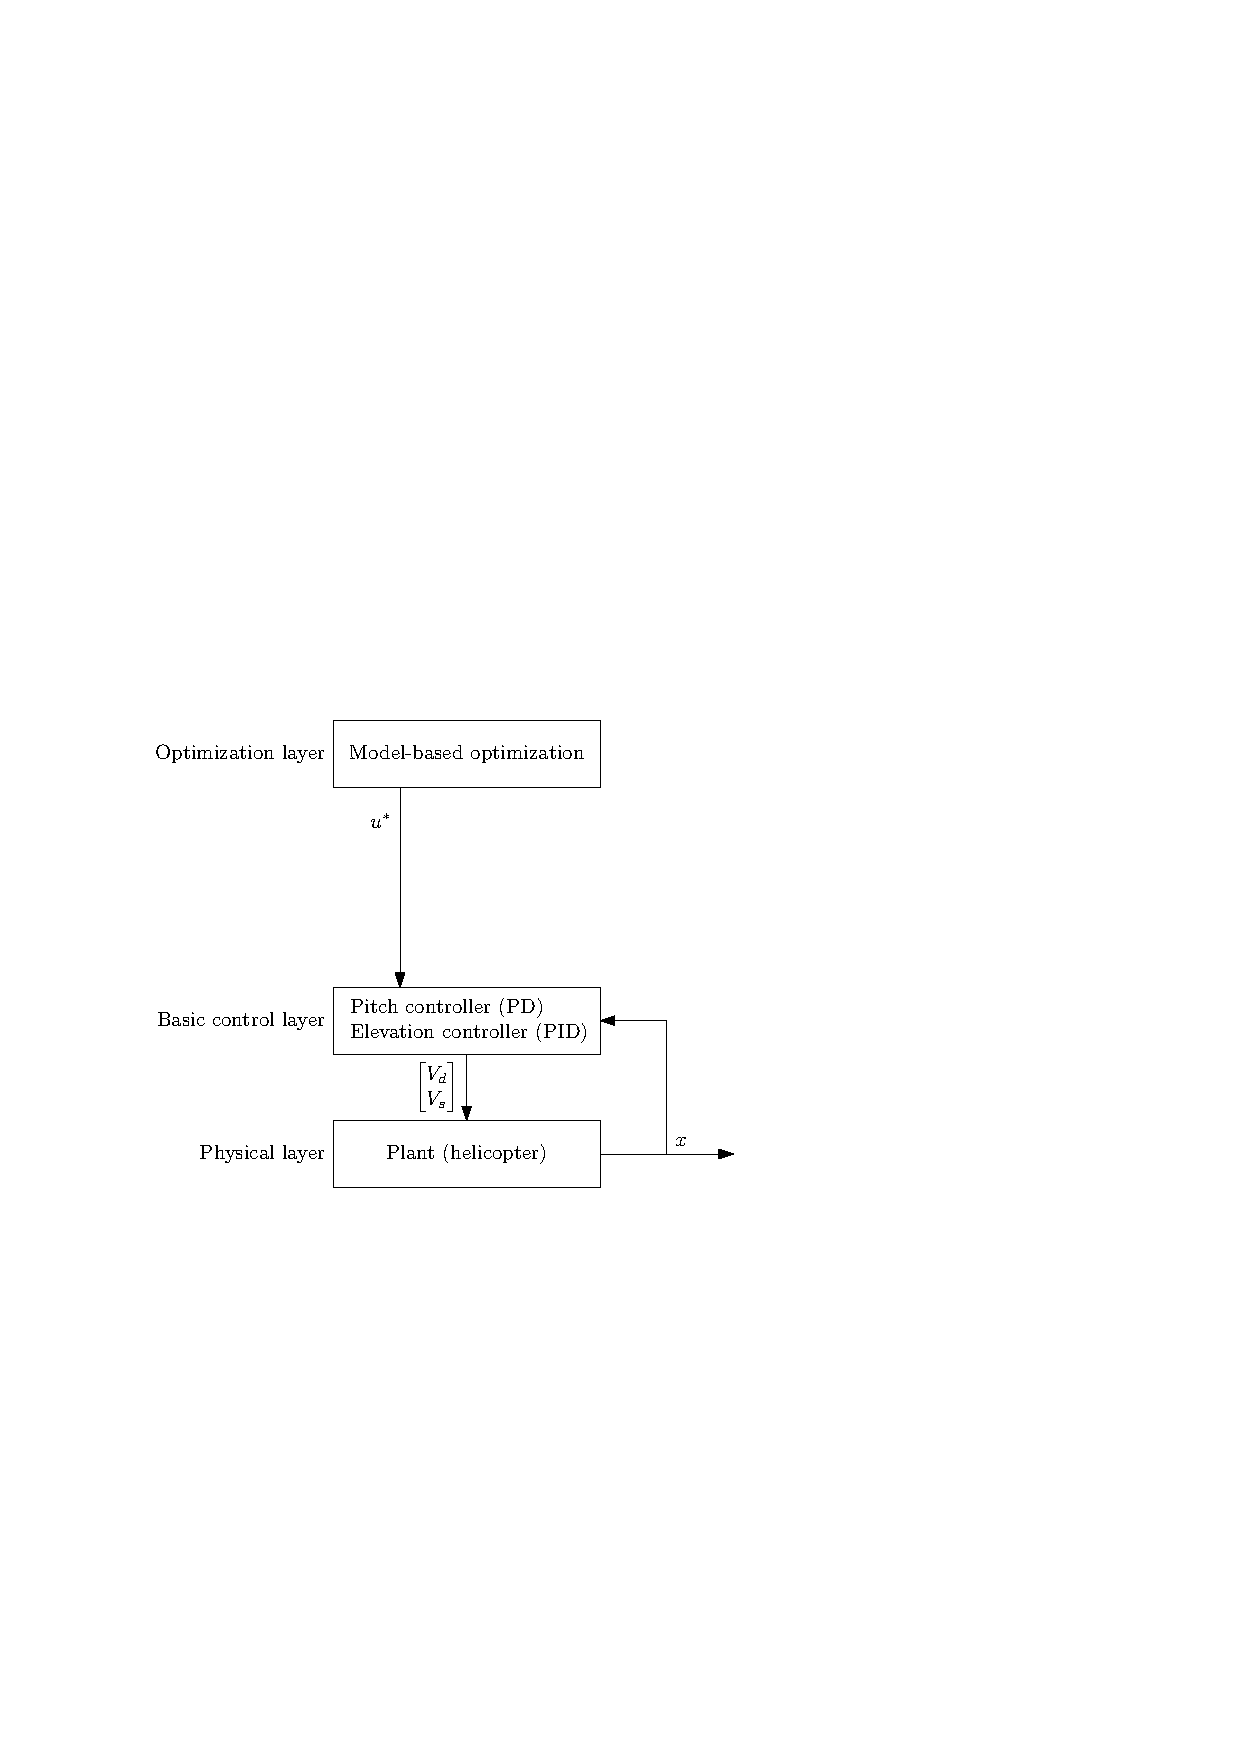
\includegraphics[width=1.00\textwidth]{figures/layers_openloop.pdf}
	\caption{A figure created with Ipe.}
	\label{fig:layers_openloop}
\end{figure}

\subsection{State space model}
From the model equations in \eqref{eq:model} we get the continuous state space equation
\begin{equation*}
	\begin{bmatrix}
		\dot{\lambda}\\
		\dot{r}\\
		\dot{p}\\
		\ddot{p}
	\end{bmatrix} = 
	\begin{bmatrix}
		0 & 1 & 0 & 0 \\
		0 & 0 & -K_2 & 0 \\
		0 & 0 & 0 & 1 \\
		0 & 0 & -K_1K_{pp} & -K_1K_{pd}
	\end{bmatrix}
	\begin{bmatrix}
		\lambda	\\
		r		\\
		p		\\
		\dot{p}
	\end{bmatrix} +
	\begin{bmatrix}
		0 \\
		0 \\
		0 \\
		K_1K_{pp} \\
	\end{bmatrix}
	p_c
\end{equation*}

or, alternatively
\begin{equation*}
	\begin{bmatrix}
		\dot{\lambda}\\
		\dot{r}\\
		\dot{p}\\
		\ddot{p}
	\end{bmatrix} = 
	\begin{bmatrix}
		0 & 1 & 0 & 0 \\
		0 & 0 & -0.0663 & 0 \\
		0 & 0 & 0 & 1 \\
		0 & 0 & -5.3095 & -0.9481
	\end{bmatrix}
	\begin{bmatrix}
		\lambda	\\
		r		\\
		p		\\
		\dot{p}
	\end{bmatrix} +
	\begin{bmatrix}
		0 \\
		0 \\
		0 \\
		5.3095 \\
	\end{bmatrix}
	p_c
\end{equation*}

However, in an effort to achieve a more accurate model, alternative state space equations are developed from estimated transfer functions based on measured step response output.

Discuss: 2 pole vs 3 pole, include transfer functions...Not exactly sure exactly what decided on, and how the model got these parameters...

\begin{equation*}
	\begin{bmatrix}
		\dot{\lambda}\\
		\dot{r}\\
		\dot{p}\\
		\ddot{p}
	\end{bmatrix} = 
	\begin{bmatrix}
		0 & 1 & 0 & 0 \\
		0 & -0.03 & -0.39 & 0 \\
		0 & 0 & 0 & 1 \\
		0 & 0 & -7.13 & -3.6
	\end{bmatrix}
	\begin{bmatrix}
		\lambda	\\
		r		\\
		p		\\
		\dot{p}
	\end{bmatrix} +
	\begin{bmatrix}
		0 \\
		0 \\
		0 \\
		6.74 \\
	\end{bmatrix}
	p_c
\end{equation*}

Discuss differences with textbook model

\subsection{Discretization}

\subsection{Optimal trajectory}

Here is a matrix equation you can use as a template:
\begin{equation}
\begin{bmatrix}
 1 &  0 &  0 & 0 & -b &  0 &  0 &  0 \\
-a &  1 &  0 & 0 &  0 & -b &  0 &  0 \\
 0 & -a &  1 & 0 &  0 &  0 & -b &  0 \\
 0 &  0 & -a & 1 &  0 &  0 &  0 & -b                                
\end{bmatrix}
\begin{bmatrix} x_1 \\ x_2 \\ x_3 \\ x_4 \\ u_0 \\ u_1 \\ u_2 \\ u_3 \end{bmatrix}
=
\begin{bmatrix}
ax_0 \\ 0 \\ 0 \\ 0      
\end{bmatrix}
\end{equation}

\subsection{Results and discussion}

\begin{figure}[htb]
	\centering
		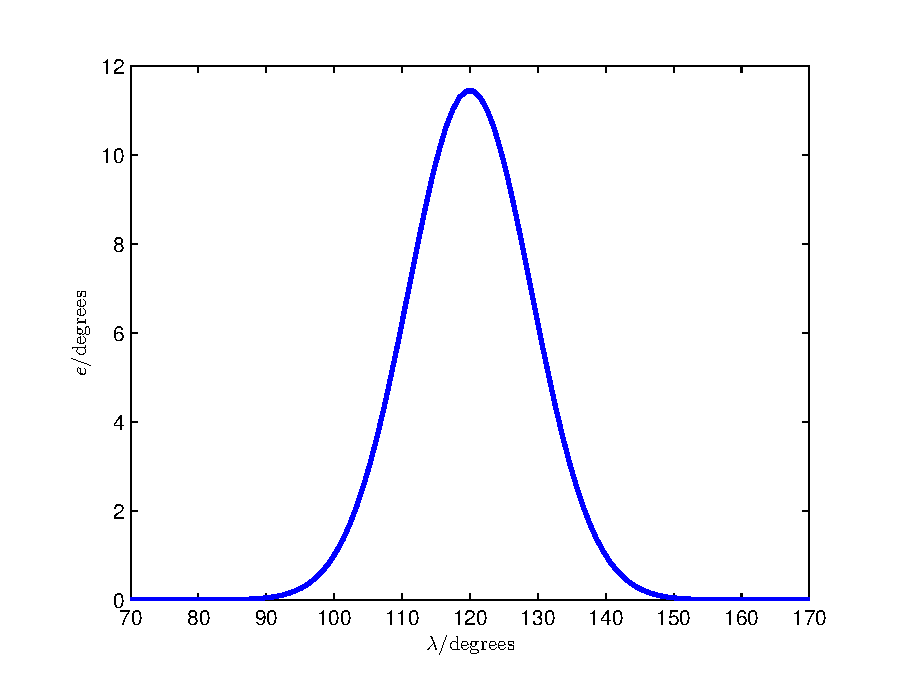
\includegraphics[width=0.8\textwidth]{figures/constraint_eps.eps}
	\caption{A plot in EPS format --- a much better idea.}
	\label{fig:constraint_eps}
\end{figure}
